\documentclass[11pt]{extarticle}
\usepackage[utf8]{inputenc}
\usepackage{cite}
\usepackage{float}
\usepackage{graphicx}
\usepackage{caption}
\usepackage{a4wide}
\usepackage{amsmath}
\usepackage{subcaption}
\usepackage{hyperref} % hyperlinks
\usepackage{url} % simple URL typesetting
\usepackage{graphicx} % more modern
\usepackage{booktabs} % professional-quality tables
\usepackage{amsfonts} % blackboard math symbols
\usepackage{microtype} % microtypography
\usepackage[nottoc]{tocbibind}
\usepackage{tikz}
\usepackage{amssymb}
\usepackage{float}
\usepackage[ruled]{algorithm2e}
\setlength\parindent{0pt}
\usepackage{geometry}
\geometry{a4paper, top=2.5cm, left=2.5cm, right=2.5cm, bottom=2.5cm}

\title{\huge \emph{Algorithmic Methods of Data Mining} \\ CS-E4600 \vspace{1cm} \\ Programming Project: \\ Graph Clustering into communities \vspace{1cm}}

\author{
Alvaro Órgaz Expósito \\ Student number: 802101 \\ \texttt{alvaro.orgazexposito@aalto.fi}   
\and
Adrià Cabeza Sant'Anna \\ Student number: 784546 \\ \texttt{adria.cabezasantanna@aalto.fi} 
\vspace{1cm}
}

\begin{document}
\maketitle
\begin{center}
\vspace{\fill} 
\includegraphics[scale=0.3]{figures/AaltoLogo.png} \vspace{5cm}
\end{center}
\newpage
\tableofcontents
\newpage

\section{Introduction}

The following report describes the analysis and explanation of diverse methods used for the following graph partitioning task.\\

Given an undirected graph $G=(V,E)$ and an integer $k > 1$ we want to partition the set of vertices $V$ into $k$ communities $V_1,...,V_k$, so that $\bigcup_{i=1}^{k} V_i = V$ and $V_i \cap V_j = \emptyset$ for all $i \neq j$. We want the communities $V_1,...,V_k$ to be as much separated from each other as possible. We also want that the communities have roughly equal size. Thus, we will evaluate the goodness of a partition $V_1,...,V_k$ using the following objective function:

\begin{equation}
\phi\left(V_{1}, \ldots, V_{k}\right)=\sum_{i=1}^{k} \frac{\left|E\left(V_{i}, \bar{V}_{i}\right)\right|}{\left|V_{i}\right|}
\end{equation}

where for $S, T \subseteq V$ with $S \cap T = \emptyset$ we define $E(S,T)$ to be the set of edges of $G$ with one endpoint in $S$ and the other endpoint in $T$, i.e., $E(S, T)=\{(u, v) \in E | u \in S \text { and } v \in T\}$, and we also  define $\bar{V}_{i}=V \backslash V_{i}$.\\

The graphs that will be used are the largest connected component of 5 graphs from the Stanford Network Analysis Project (SNAP): 

\begin{table}[h]
\centering
\begin{tabular}{|l|l|l|l|}
\hline \textbf{Graph} & \textbf{\#vertices} & \textbf{\#edges} & \textbf{\#clusters} \\ \hline
ca-GrQc & 4158 & 13428 & 2 \\ \hline
Oregon-1 & 10670 & 22002 & 5 \\ \hline
soc-Epinions1 & 75877 & 405739 & 10 \\ \hline
web-NotreDame & 325729 & 1117563 & 20 \\ \hline
roadNet-CA & 1957027 & 2760388 & 50 \\ \hline
\end{tabular}
\caption{Graphs statistics.}
\end{table}

\section{Literature review}

The task of partitioning a graph has grown quite popular since we find ubiquitously in real-world network several sets of densely connected nodes, joined by a small number of edges. Moreover, as it can be seen in Figure [\ref{drawing}], this task is not trivial at all as normally no clear partitions are found in the graph, in fact, graph partitioning is an NP-hard problem. Therefore, there are a lot of different approaches to tackle the problem, so in the following section we will introduce some of them in order to get an essential view of the problem and its complexity before implementing our methods.

\begin{figure}[h]
\centering
\includegraphics[scale=0.03]{figures/ca-GrQc_spring_only_nodes_graph.jpg}
\caption{Spring representation of the ca-GrQc graph.}
\label{drawing}
\end{figure}

\subsection{The Girvan-Newman method}

The method introduced in 2002 by Girvan M. and Newman M. \cite{Girvan2002} is based on the fact that edges connecting communities should have high \textbf{betweenness centrality} which means that for every pair of vertices in a connected graph, there exists at least one shortest path. The betweenness centrality for each vertex is the number of shortest paths that pass through the vertex. Therefore, it removes links in order to decrease betweenness and returns the remaining components of the network as the communities obtained. Its main downside is that it makes heavy demands on computational resources, running in $\mathcal{O}(m^2n)$ with $m$ edges and $n$ vertices or $\mathcal{O}(n^3)$ on a sparse graph.

\begin{figure}[h]
\centering
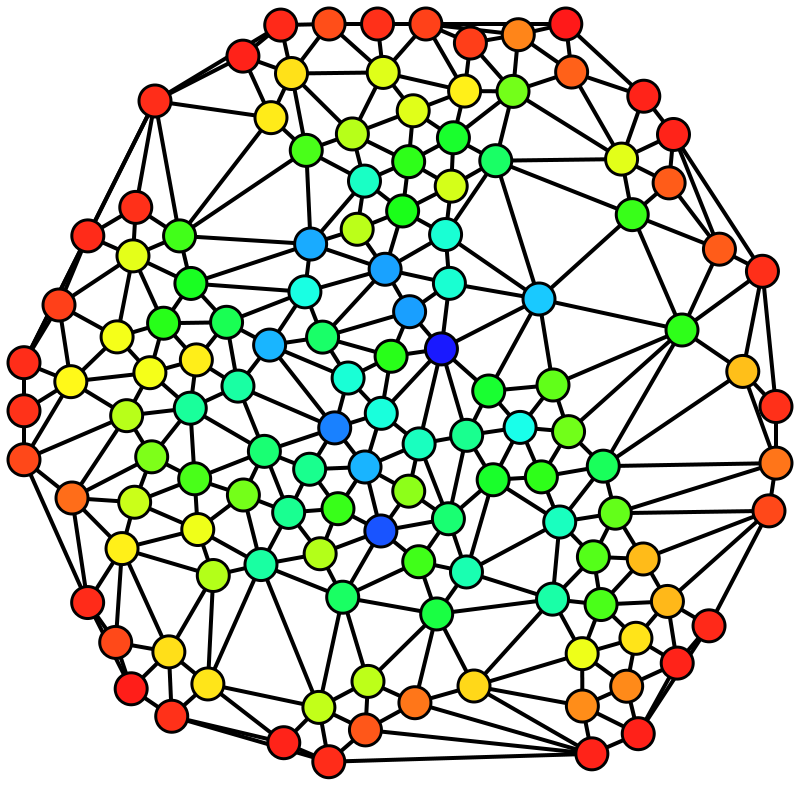
\includegraphics[width=0.3\linewidth]{figures/graph_betweenness.png}
\caption{An undirected graph colored based on the betweenness centrality of each vertex from least (red) to greatest (blue). Source: Wikipedia.}
\label{girvan_newman}
\end{figure}
\bigskip

\begin{algorithm}[H]
\begin{enumerate}
    \item Calculate the betweenness for all edges in the network.
    \item Remove the edge with the highest betweenness.
    \item Recalculate betweennesses for all edges affected by the removal.
    \item Repeat from step 2 until no edges remain.
\end{enumerate}
\caption{The Girvan-Newman method.}
\end{algorithm}

\subsection{CNM method}

The Clauset, Newman and Moore (CNM) method \cite{cond-mat/0408187} is based on increasing \textbf{modularity} of a network. The modularity is an evaluation metric for community detection and it tests a given division of a network against the random division. The algorithm measures when a division is a good one, in the sense that there are many edges within communities and only a few between them. It starts with $N$ communities and at every step of the algorithm two communities that contribute maximum positive value to global modularity are merged.

\subsection{Spectral methods}

Spectral clustering methods use the spectrum of a graph to perform dimensionality reduction before clustering in fewer dimensions. It is better to use this approach than directly using K-means because K-means performs poorly since it can only find spherical clusters. The idea is based on computing the eigenvectors corresponding to the second-smallest eigenvalue of the normalized Laplacian or some eigenvector of some other matrix representing the graph structure \cite{belkin2003laplacian},\cite{0711.0189},\cite{ng2002spectral}. The resulting eigenvector is used as a vertex embedding of the graph to determine the clustering. Its main downside is that computing eigenvalues and eigenvectors for graphs are slow and hence such methods might face scalability issues when applied to massive graphs. Normally, one common way to tackle this problem is to use the more efficient method \textit{Implicitly Restarted Lanczos} where only the $k$ largest or smallest eigenvalues and its eigenvectors are needed.\\

For example, if a graph $G$ is a collection of $k$ disjoint cliques, the normalized Laplacian is a block-diagonal matrix that has eigenvalue zero with multiplicity $k$ and the corresponding eigenvectors serve as indicator of the membership of each clique: the eigenvector $v_i$ has a different value or a larger magnitude for the vertices that are inside the clique $i$ than the other vertices. Thus, there is an underlying structure that can be seen using the eigenvectors of the Laplacian. Moreover, if we introduce edges between the cliques we will find that $k-1$ of the $k$ eigenvalues that were zero will become slightly larger than zero so it is a robust method. 

\subsubsection{Recursive Spectral Bi-partitioning}

This method uses one of the typical ideas of spectral clustering: computing the eigenvector corresponding to the second-smallest eigenvalue of the normalized Laplacian. The resulting eigenvector works like an embedding of the vertices to split the graph into two clusters: a positive value in the $i$ position of the eigenvector indicates that the vertex $i$ belongs to a cluster $C_1$ and a negative value that it belongs to a cluster $C_2$.\\

In order to do more than two partitions, we can perform a two-classification iteratively, using the spectra of the resulting induced subgraphs. This will yield a divisive hierarchical clustering algorithm that we will call Recursive Spectral Bi-partitioning.\\

\begin{algorithm}[h]
\textbf{Input}: A graph $G$ and the desired clusters $k$\\
\textbf{Pre-processing}: Build Laplacian matrix $L$ of the graph\\
\textbf{Decomposition}:
\begin{itemize}
    \item[-] Find eigenvectors $X$ and eigenvalues $\lambda$ of the matrix $L$
    \item[-] Sort the eigenvalues:  $\lambda_1 < \lambda_1 < \lambda_2 ... < \lambda_n$
    \item[-] Map vertices to corresponding components of the eigenvector corresponding to $\lambda_2$
\end{itemize}
\textbf{Grouping}:
\begin{itemize}
    \item[-] Sort components of reduced 1-dimensional vector
    \item[-] Identify clusters by splitting the sorted vector into two: negative and positive 
    \item[-] Induce two subgraphs using the clusters identified
\end{itemize}
\textbf{Recurse with the induced subgraphs until $k$ partitions are reached}
\caption{Recursive Spectral Bi-partitioning algorithm.}
\end{algorithm}

\subsubsection{K-Way Spectral Clustering}

Another popular method to tackle the multicluster problem that is more commonly used is the so-called K-way Spectral Clustering introduced by Jianbo Shi and J. Malik \cite{JianboShi2000}.\\

This method instead of using only the eigenvector associated to $\lambda_2$ from the Laplacian matrix it uses multiple eigenvectors to build a reduced space where some structural information is conserved. Afterwards, any multidimensional clustering algorithm can be performed such as KMeans.\\

\begin{algorithm}[H]
\textbf{Input}: A graph $G$ with $n$ nodes and the desired clusters $k$\\
\textbf{Pre-processing}: Build Laplacian matrix $L$ of the graph\\
\textbf{Decomposition}:
\begin{itemize}
    \item[-] Find eigenvectors $X$ and eigenvalues $\lambda$ of the matrix $L$
    \item[-] Build embedded space from the eigenvectors corresponding to the $k$ smallest eigenvalues
\end{itemize}
\textbf{Clustering}:
\begin{itemize}
    \item[-] Apply KMeans to the reduced $n \times k$ space to produce $k$ clusters
\end{itemize}
\label{kway-spectral}
\caption{K-way Spectral Clustering algorithm.}
\end{algorithm} \vspace{0.5cm}

\section{Implemented algorithmic approaches}

Our approach is based on the algorithm [\ref{kway-spectral}] mentioned in the previous section. We have started implementing the algorithm on Python3 using \textbf{numpy} for basic mathematical operations, \textbf{networkx} to deal with the graphs in a sparse way and create their adjacency matrix as well as the normalized Laplacian matrix, \textbf{sklearn} for the KMeans algorithm with default KMeans++ centroids initialization as well as Euclidean distance, and \textbf{scipy} for the eigendecomposition. Also, we have implemented the target score function to score the clustering output.\\

Our first implementation was not able to do the eigendecomposition for the largest graphs because we were not using sparse matrices. For the largest graph, roadNet-CA, we had to create an adjacency matrix of $1957027^2 \times 4B$  ($V^2 \times$ bytes of an integer) $ = 14268$ GB of memory. However, we noticed that thes graphs are very sparse since the number of edges is highly smaller that $V^2$, so the first improvement we made was using sparse matrices.\\

After implementing this improvement, we have added several different configurations and parameters to customize the algorithm and develop deep experiments and find the optimal solutions for all the graphs. This is the list of the principal extensions or added options which can be found in the parameters of the main Python script \textit{graph\_clustering.py}:
\begin{itemize}
    \item Compute the adjacency and Laplacian matrixes manually using sparse functions with the package \textbf{scipy} instead of using already implemented functions from \textbf{networkx}.
    \item Compute the unnormalized Laplacian matrix.
    \item Normalize the eigenvectors by nodes or by eigenvectors axis.
    \item Invert the eigenvectors multiplying by -1 the Laplacian matrix and selecting the eigenvectors with higher eigenvalues.
    \item Select only the second eigenvector as an embedding (only 1 dimension by node) for the graph clustering.
    \item Different clustering methods: KMeans from \textbf{scipy} and {sklearn}, XMeans and Hierarchical Agglomerative Clustering from \textbf{pyclustering} and KMeans from \textbf{pyclustering} for a more customized version of the algorithm. Note that we use the default Euclidean distance metric and centroids initialization for all the clustering methods except the KMeans method from pyclustering.
    \item Iterate different random seeds for the selected clustering method and store its best output.
    \item Customized distance metrics (Minkowski, Chebyshev, Euclidean) and centroids initialization (random and based on KMeans++ algorithm) for the \textbf{pyclustering} KMeans option.
\end{itemize}

Note that there are several ways to compute the Laplacian matrix but we have considered two versions:
\begin{itemize}
    \item Unormalized: $L_{u}=D-A$
    \item Normalized: $L=I-D^{-1/2} A D^{-1/2}$
\end{itemize}

\section{Experimental results}

\label{results}

Since we have been competing in the competition and we have implemented several options and parameters to try for our approach, we have done a wide range of experiments and trials. In this section, we are going to define and explain a concrete experiment which is useful to understand behaviours and make comparisons. However, before introducing it we explain the main conclusions after using and tuning the approach parameters.
\begin{itemize}
    \item When computing the Laplacian with \textbf{networkx}, we observe a trade-off between duration and performance since by using the unnormalized option it takes way more time but it leads to way better score function results when clustering. The reason why we are getting so much better scores is that the unnormalized Laplacian serves in the approximation of the minimization of our objective function as it is shown in \cite{buger_2015}. 
    \item We obtain better results without eigenvectors normalization but without big differences comparing to normalizing by embedding (rows). However, we get very bad results when normalizing by eigenvectors (columns).
    \item When trying to use only the second smallest eigenvector we get very decent results, very competitive when comparing to keeping more eigenvectors.
    \item When inverting the Laplacian matrix as mentioned before, we do not improve performance.
    \item The number of eigenvectors kept is very important and we have played with selecting less and more than $k$, which leads to the top 10 results in the competition.
    \item By computing the Laplacian matrix manually instead of using the module \textbf{networkx} we do not observe differences.
    \item By iterating through different seeds we get different results for the same configurations and clustering methods, that is why we played with this parameter too in the competition.
\end{itemize}

Now, we explain and give numerical conclusions of the main experiment. By fixing some parameters we have tried all implemented clustering methods and in the case of the customized KMeans with \textbf{pyclustering} we test three different distance metrics as well as different centroids initializations randomly or with KMeans++. The rest fixed parameters are: number of unnormalized eigenvectors, unnormalized Laplacian with \textbf{networkx}, and seed 0. Due to the time restrictions and the fact that the biggest graphs are really time consuming, we have developed the experiment on the two smaller graphs.\\

On the other hand, we have set a baseline output for each graph which corresponds to a random cluster assignation of each node. This baseline was useful in the beginning of our experiments in order to see whether we were improving a trivial solution. The score function results achieved by it are:
\begin{itemize}
    \item ca-Qrc: 6
    \item Oregon-1: 15
    \item soc-Epinions1: 90
    \item web-Notredame: 120
    \item roadNet-CA: 100
\end{itemize}

In the following tables, you can find the experiment results. Note that d1, d2, d3 refer to Minkowski, Chebyshev, Euclidean and c1, c2 refer to random and KMeans++ centroids initialization and the time and memory usage stated on the table is without taking in account the computation of the eigenvectors of the laplacian since this is only calculated once, saved as a pickle file and used by all the methods.

\begin{table}[H]
\centering
\begin{tabular}{|c|c|c|c|c|c|}
\hline
\textbf{Method} & \textbf{Score} & \textbf{Memory} & \textbf{Time} \\ \hline
KMeans \textbf{pyclustering} d1 c1  & 0.118  & 139.844 MiB & 1.243 seconds\\ \hline
KMeans \textbf{pyclustering} d1 c2 & 0.154 & 140.078 MiB & 1.778 seconds \\ \hline
KMeans \textbf{pyclustering} d2 c1 & 0.200 & 139.941 MiB & 1.258 seconds \\ \hline 
KMeans \textbf{pyclustering} d2 c2 & 0.159 &  140.188 MiB & 1.861 seconds\\ \hline
KMeans \textbf{pyclustering} d3 c1 & 0.200 & 139.871 MiB  &  1.534 seconds\\ \hline
KMeans \textbf{pyclustering} d3 c2 & 0.084 & 139.914 MiB  & 1.196 seconds \\ \hline
KMeans \textbf{scipy} & 0.172 & 134.125 MiB & 1.644 seconds\\ \hline
KMeans \textbf{sklearn} & 0.063 & 136.433 MiB & 0.505 seconds\\ \hline 
XMeans \textbf{pyclustering} & 0.084 &  139.652 MiB & 1.724 seconds\\ \hline
Agglomerative \textbf{pyclustering} & 0.125  & 139.387 MiB & 275.884 seconds\\ \hline
\end{tabular}
\caption{Experiments on graph \textit{ca-GrQc} taking 10 eigenvectors as a high-dimensional embedding.}
\label{caQrc}
\end{table}

\begin{table}[H]
\centering
\begin{tabular}{|c|c|c|c|c|c|}
\hline
\textbf{Method} & \textbf{Score} & \textbf{Memory} & \textbf{Time}\\ \hline
KMeans \textbf{pyclustering} d1 c1 & 0.990 & 157.027 MiB & 0.465 seconds\\ \hline
KMeans \textbf{pyclustering} d1 c2 & 1.361 & 158.105 MiB  &  0.502 seconds \\ \hline
KMeans \textbf{pyclustering} d2 c1 & 1.631 & 157.301 MiB  & 0.435 seconds\\ \hline
KMeans \textbf{pyclustering} d2 c2 & 1.818 & 158.180 MiB & 0.477 seconds\\ \hline
KMeans \textbf{pyclustering} d3 c1 & 0.867 &  158.203 MiB & 0.434 seconds\\ \hline 
KMeans \textbf{pyclustering} d3 c2 & 1.217 & 157.934 MiB &  0.477 seconds\\ \hline
KMeans \textbf{scipy} & 1.449 & 142.039 MiB & 0.978 seconds \\ \hline
KMeans \textbf{sklearn} & 0.654 & 145.930 MiB & 1.059 seconds \\ \hline
XMeans \textbf{pyclustering}  & 0.867 & 156.879 MiB & 0.484 seconds \\ \hline
\end{tabular}
\caption{Experiments on graph \textit{Oregon-1} taking 13 eigenvectors as a high-dimensional embedding.}
\label{Oregon1}
\end{table}

From table [\ref{caQrc}] we can see that the Agglomerative Hierarchical clustering takes much more time than the other approaches and does not compute a better partition, hence we decided not to push forward with this method for the other graphs. We can also observe in tables [\ref{caQrc}], [\ref{Oregon1}] how sklearn is the method that gives us the best score. We believe that the reason of having different scores between different KMeans methods could be the way some parameters are implemented in every library such as tolerance or number of maximum iterations. Moreover, in terms of memory usage, we do not observe a huge difference between methods (all of them are using sparse matrices) even though they come from different libraries.\\

The next tables were calculated only using the sklearn method and varying the number of smallest eigenvectors we keep as a high-dimensional embedding of the graph. Here we can see how much this value changes the outcome of score.

\begin{table}[H]
\centering
\begin{tabular}{|c|c|c|c|c|c|}
\hline
\textbf{\# Smallest Eigenvectors} & \textbf{Score} \\ \hline
1  & 6.5424  \\ \hline
2-8 & 0.0836 \\ \hline
9-10 & 0.0627\\ \hline
\end{tabular}
\caption{Experiments on graph \textit{ca-GrQc} on how taking different number of eigenvectors as a high-dimensional embedding changes outcome.}
\end{table}

\begin{table}[H]
\centering
\begin{tabular}{|c|c|c|c|c|c|}
\hline
\textbf{\# Smallest Eigenvectors} & \textbf{Score} \\ \hline
3 &  1.110\\ \hline
6 &  0.7220\\ \hline
9  & 0.6639 \\ \hline 
12-18  & 0.6341 \\ \hline
\end{tabular}
\caption{Experiments on graph \textit{Oregon-1} on how taking different number of eigenvectors as a high-dimensional embedding changes outcome.}
\end{table}

The experiments were run in a server called \textit{brute.aalto.fi} provided by Aalto University with the following characteristics:
\begin{itemize}
    \item  32 Intel(R) Xeon(R) CPU E5-2670 0 @ 2.60GHz x86\_64 Architecture
    \item  256 GiB System memory
\end{itemize}

\section{Competition results}

In this section, we will explain our optimal configuration and output by graphs which correspond to our final competition submission. We have tried several configurations and combinations of parameters (explained in previous sections), mainly including different numbers of eigenvectors kept for the clustering algorithms and different seeds, which has been the key to get top 10 positions in the competition.\\

We have used the following same parameters for all of them: clustering method KMeans \textbf{sklearn} which as mentioned before uses Euclidean distance and KMeans++ centroids initialization, computation of Laplacian matrix with \textbf{networkx} without normalization and without inverting, neither eigenvectors normalization. Moreover, in the following table you can find the number of smallest eigenvectors kept and random seed for each graph, as well as the score and final position in the competition.

\begin{table}[H]
\centering
\begin{tabular}{|l|l|l|l|l|}
\hline
\textbf{GraphID} & \textbf{Eigenvectors} & \textbf{Seed} & \textbf{Score} & \textbf{Position}\\ \hline
ca-Qrc & 10 & 0  & 0.0627414293 & 1\\ \hline
Oregon-1 & 13 & 1 & 0.6003758692 & 1\\ \hline
soc-Epinions1 & 27 & 8 & 0.5503901003 & 8\\ \hline
web-Notredame & 60 & 0 & 0.0306827622 & 12\\ \hline
roadNet-CA & 100 & 0 & 0.2626139803 & 14\\ \hline
\end{tabular}
\end{table}

\section{Conclusions}

Overall, we can conclude that we have implemented successfully different methods to partition large networks and we have experienced empirically how useful can be to use the properties found in the spectra of a graph. We also have learnt the hard way how difficult can be to work with large networks in terms of time and memory usage; in fact, some of our first approaches which involved Hill Climbing and Simulated Annealing methods were too harsh to implement in this kind of networks.\\

Furthermore, as it can be seen in the section [\ref{results}], we have also observed how clustering on a higher dimensional space than the one stated in the original algorithm [\ref{kway-spectral}], that is to say taking more eigenvectors than $k$, gave us better results. We hypothesize that this is because the additional eigenvectors provide more additional information of the structure of the graph.  

\newpage

\bibliography{bibliography.bib}  
\bibliographystyle{ieeetr}

\end{document}